%Lorem ipsum dolor sit amet.
\subsection{Global Descriptor Table}
\subsubsection{Descriptores de código y datos}
Antes de pasar a modo protegido creamos cuatro descriptores de segmento en la GDT. Como nos piden que dejemos lugar para 7 descriptores al comienzo de la tabla empezamos en índice 8, dejando libres índices desde 0 a 7.
Los descriptores están dados por dos doble words (ver Figura 1), una doble word ocupa 32 bits, y se representan con estructuras llamadas \verb|str_gdt_entry|, donde cada campo de la estructura representa subconjunto de bits de cada una de las dos doble words. En lo que sigue nos referiremos a los bits de las doble words.\\
\begin{figure}[h]
\centering
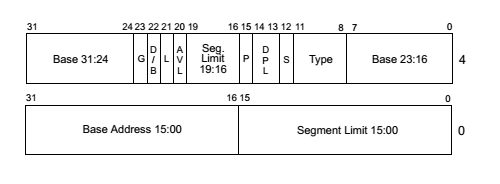
\includegraphics[scale=0.6] {descriptor_segmento}
\caption{Descriptor de segmento (primera doble word abajo y segunda doble word arriba).}
\end{figure} 

 Los descriptores de código, ubicados en índice 8 y 10 de tabla, se completan tal que los bits de $BASE$, que son los bits 16 a 31 de primer doble word junto a bits 0 a 7 y bits 24 a 31 de segunda doble, queden todos en 0. Esto a causa de que debemos direccionar los primeros 500 megabytes de memoria y por lo tanto la base de los segmentos es 0. Luego el límite debe indicar 500 megas y por lo tanto debemos setear el bit $G$, granularidad, que es el bit número 23 de segunda doble word. A causa de esto el límite tiene rango desde 4 Kbytes a 4 Gbytes. Entonces despejando de ecuación $Limite$ * \verb|0x400| + \verb|0x3FF| = 500 $megas$ se obtiene valor de  \verb|0x7CFFF|. Escribimos en bits 0 a 15 de primer doble word, campo de límite, el valor \verb|0xCFFF| y completamos el campo de límite escribiendo en los bits 16 a 19 de segunda doble word el valor \verb|0x7|. Luego seteamos los bits de tipo, bits 8 a 11 en segunda doble word, de manera que indique que el descriptor es de código y se permite ejecución y lectura. Esto se hace llenando esos bits con \verb|0xA|. Paso seguido seteamos bit $S$, bit 12 en segunda doble word, especificando que desciptor no es de sistema. Pasamos a bits 13 a 14 en segunda doble word, $DPL$, en donde establecemos privilegios. Acá llenamos con dos ceros en caso de descriptor de nivel 0 mientras que para descriptor de nivel 3 llenamos los bits con dos unos. Luego Seteamos bit $P$, número 15 en segunda doble word, tal que indique que el descriptor está presente, sino al buscar dirección no se encontraría el descriptor y se generaría una falta. Bits $AVL$ y $L$, bits 20 y 21 respectivamente de segunda doble word, se dejan en cero indicando no segmento de 64 bits. Finalmente bit $D/B$, bit 22 en segunda doble word, se setea indicando operaciones en 32 bits.\\
\indent En los descriptores de datos todos los bits menos los de tipo se completan exactamente como completamos los de código, llenando los bits $DPL$ con ceros para segmento de datos nivel 0 y con unos para el de nivel 3. Los bits de tipo se llenan con \verb|0x2| tal que indican segmento de datos para lectura y escritura. Estos descriptores están en los índices 9 y 11 de tabla.\\
\indent Para descriptor de segmento de pantalla debemos especificar como base \verb|0xB8000| y para el límite necesitamos resolver (80 * 50 * 2) - 1, donde 80 es la cantidad de celdas, 1 celda == 2 bytes, en fila de pantalla y 50 es cantidad de celdas en columna. Es decir que el límite nos la cantidad de bytes que necesitamos para escribir en cualquier parte de la pantalla. Luego el valor del límite es \verb|0x1F3F|. Este descriptor va en índice 12 de la $GDT$.\\
Comenzamos llenando los primeros bits de $BASE$, bits 16 a 31 de primer doble word, con \verb|0x8000| (parte menos significativa de base) y continuamos llenando bits 0 a 7 de segunda doble word con \verb|0x0B| y bits 24 a 31 de misma doble word en \verb|0x00| (parte más significativa de base). Paso seguido llenamos bits 0 a 16 de primera doble word con \verb|0x1F3F|, límite de segmento, y bits 16 a 19 de segunda doble word en 0. Luego llenamos bits de tipo con \verb|0x2| indicando segmento de datos permitiendo lectura y escritura. Seguimos con bit $S$ puesto en cero indicando que el segmento no es de sistema y bits de $DPL$ en cero para indicar privilegio 0. El bit $P$ es seteado para especificar segmento como presente y bits $AVL$ y $L$ en cero, el primero no es usado y el segundo indica no segmento de 64 bits. Finalizamos seteando bit $D/B$, para indicar operaciones en 32 bits, y bit $G$ en 0 porque el límite es menor a 1 Mbyte.

%\begin{verbatim}
 % Your text here.
%\end{verbatim}

\subsubsection{Pasaje a modo protegido y pila de kernel}
En \verb|kernel.asm| cargamos el registro $GDTR$ con dirección de tabla, que es arreglo de\\ \verb|str_gdt_entry|, usando instrucción \verb|lgdt|. Luego llamamos a función \verb|habilitar_A20| y seteamos el bit $PE$ del registro $CR0$. Esto se hace moviendo $CR0$ a registro general de 32 bits, entonces aplicamos \verb|or| bit a bit entre el registro y valor 1 y movemos resultado a $CR0$. Siguiente instrucción es un salto a \verb|0x40:modoprotegido| donde \verb|0x40| es valor de selector de segmento tal que en bits 3 a 15 de selector (ver Figura 2) se escribe 8 en binario indicando índice 8 en la tabla. Por otra parte valores de bits 0 y 1, ambos en cero, de selector indican segmento con privilegio 0 y bit 2, también en cero, especifica en que tabla buscar, en este caso tabla global. Es decir buscamos segmento de código en la $GDT$ y allí seguimos en las instrucciones bajo etiqueta \verb|modoprotegido|.
\begin{figure}[h]
\centering

\includegraphics[scale=0.6] {selector_segmento}
\caption{Selector de segmento.}
\end{figure} 

El código siguiente está en 32 bits, incluyendo lo que está bajo etiqueta \verb|modoprotegido|. Allí cargamos los selectores de segmento $ds, es, ss, gs$ con \verb|0x48| tal que bits 3 a 15 de \verb|0x48| indican que cada selector indexe en descriptor número 9 de la $GDT$ (bit 2 en cero) y con privilegio 0 (bits 0 y 1 en cero). Paso seguido cargamos selector de segmento $fs$ con \verb|0x60| tal que se escribe 12 en binario en bits 3 a 16 de selector, indicando índice 12, y los bits restantes especifican buscar en $GDT$ con privilegio 0, es decir donde está el segmento de pantalla de kernel. Luego establecemos la base de la pila del kernel en dirección \verb|0x27000|, cargando registro $esp$ con esta dirección.


